% I use a custom document class that can be found at
% github.com/mwhittaker/texmf. Honestly, it's a big pain in the butt to set it
% up. Sorry this document isn't easier to compile! If you have the hw document
% class set up, you can compile this document with `latexmk -pdf answers.tex`

\documentclass{hw}
\title{CS 5220 -- 2015-09-10 Preclass Questions}

\hypersetup{
  colorlinks = true,
  allcolors = blue,
}

\begin{document}
\maketitle{}

\begin{enumerate}
  \item
    In order to draw a roofline model for the totient nodes, we need to know
    the peak memory bandwidth and the peak floating-point performance. The peak
    memory bandwidth is 59 GB/s, and the peak floating-point performance is 120
    GFLOPs/s. The roofline diagram generated from these parameters can be found
    in \figref{roofline}. With the addition of the Phi boards, the max flops
    would increase, but the memory bandwidth would remain constant.

  \item
    Imagine you have two independent processes executing on two distinct cores.
    There are some overheads in communication between the two cores whenever
    the two processes need to communicate. On the other hand, a hyperthreaded
    core can run both processes on the same core and reduce the overhead of
    communication.

  \item
   The Phi architecture arranges cores using a ring network. This means that
   memory access is non-uniform. A processor can access the memory of its
   neighbor faster than it can connect to the memory of a node on the other
   side of the ring.

  \item
    Assume we have $p$ processors, each vector is of size $n$, performing a
    flop takes time $f$, and communicating a double takes time $c$. Serially,
    the dot product takes $2nf$ time. With $p$ processors, it takes time
    $\frac{2nf}{p} + pc$ time. This is a speedup of
    \[
      \frac{2nf}{\frac{2nf}{p} + pc}
    \]
\end{enumerate}

\begin{figure}[p]
  \centering
  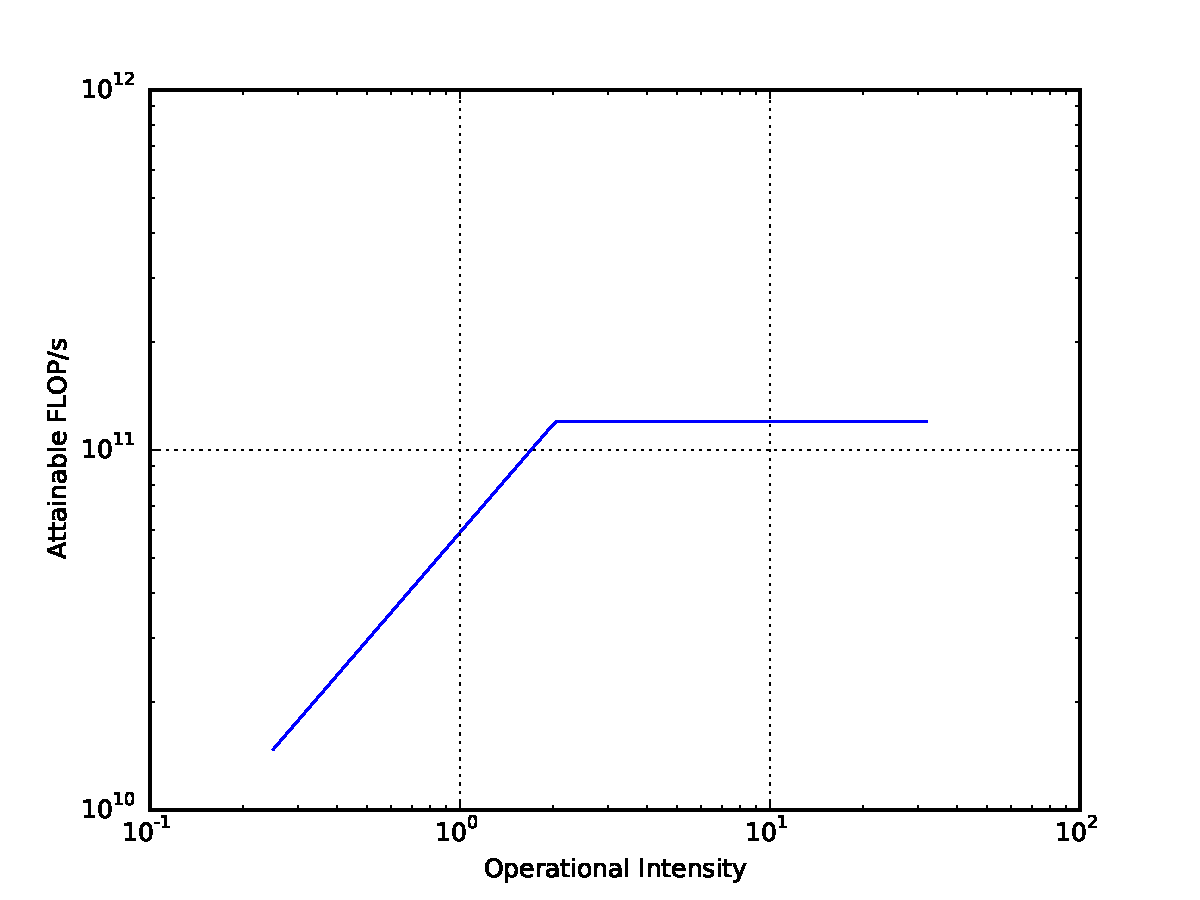
\includegraphics[width=\textwidth]{roofline.pdf}
  \caption{Roofline for Totient Node}
  \label{fig:roofline}
\end{figure}
\end{document}
